\documentclass[tikz,border=0pt]{standalone}
\usepackage{fontspec}
\IfFontExistsTF{TeX Gyre Heros}{\setmainfont{TeX Gyre Heros}}{\setmainfont{Latin Modern Sans}}
\usepackage{amsmath,amssymb,booktabs,array}
\DeclareMathSizes{9}{9}{8.6}{8.6}
\usepackage{pgfplots}
\pgfplotsset{compat=1.17}
\usetikzlibrary{arrows.meta,positioning,calc,fit,shapes.geometric,backgrounds}
\definecolor{ink}{HTML}{183247}
\definecolor{blue}{HTML}{286B91}
\definecolor{teal}{HTML}{19796F}
\definecolor{orange}{HTML}{AC671F}
\definecolor{muted}{HTML}{596C78}
\tikzset{
  every node/.style={font=\fontsize{9}{11}\selectfont,text=ink},
  arr/.style={-{Stealth[length=1.7mm]},line width=.55pt,draw=muted},
  panel/.style={draw=muted!35,line width=.5pt,rounded corners=1mm,fill=white},
  box/.style={draw=blue!70,line width=.55pt,rounded corners=.8mm,fill=blue!5,align=center,inner sep=2mm},
  label/.style={font=\fontsize{9}{11}\selectfont,align=left,inner sep=0},
  paneltitle/.style={font=\bfseries\fontsize{9.5}{12}\selectfont,anchor=west,inner sep=0}
}

\begin{document}
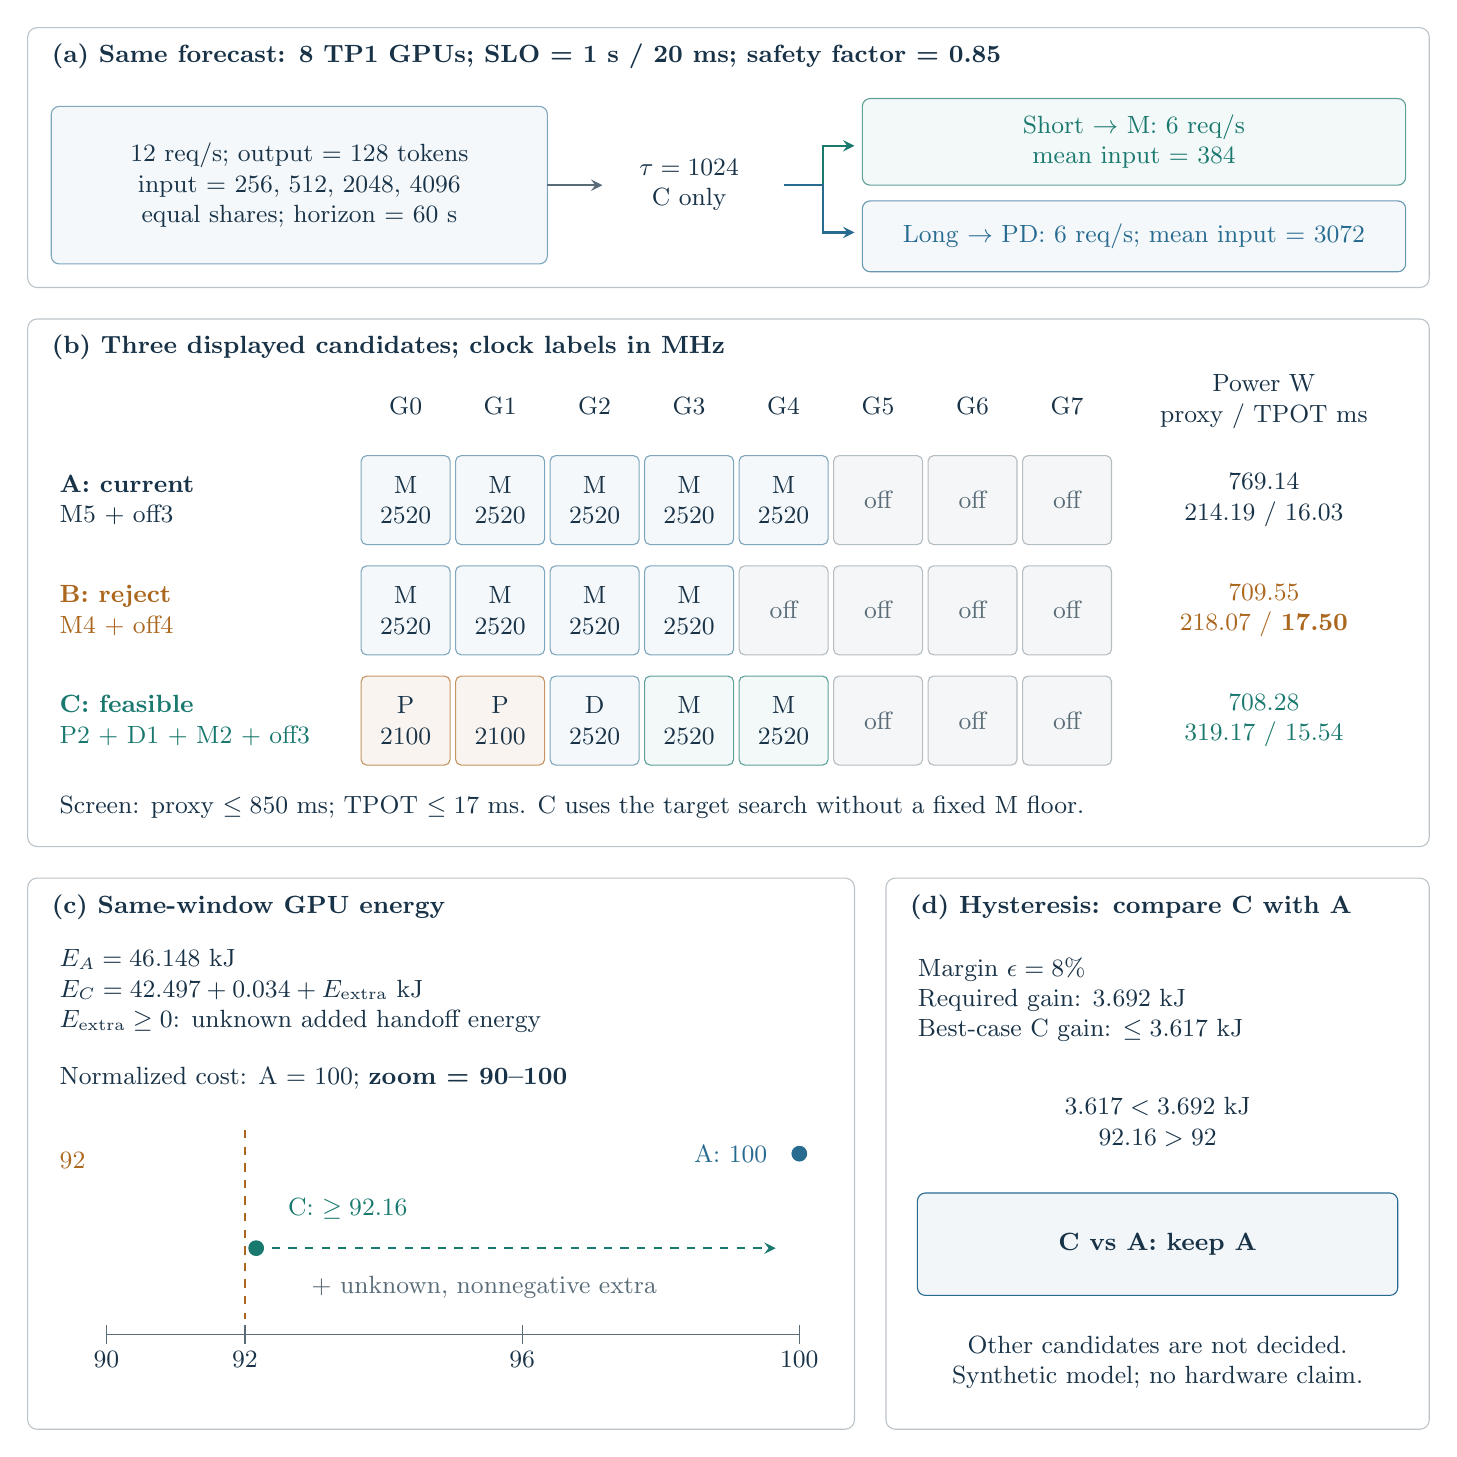
\begin{tikzpicture}[x=1mm,y=-1mm,font=\fontsize{9}{11}\selectfont,
  txt/.style={text=ink,align=left,inner sep=0pt},
  title/.style={txt,font=\bfseries\fontsize{9}{11}\selectfont},
  cell/.style={draw=blue!60,fill=blue!5,rounded corners=.7mm,minimum width=11.3mm,minimum height=11.3mm,align=center,inner sep=.3mm},
  offcell/.style={cell,draw=muted!45,fill=muted!6,text=muted}]
  \path[use as bounding box] (0,0) rectangle (178,178);

  % (a) One forecast, two conditional paths.
  \draw[draw=muted!40,fill=white,rounded corners=1.2mm] (0,0) rectangle (178,33);
  \node[title,anchor=north west] at (3,2) {(a) Same forecast: 8 TP1 GPUs; SLO = 1 s / 20 ms; safety factor = 0.85};
  \draw[draw=blue!60,fill=blue!5,rounded corners=1mm] (3,10) rectangle (66,30);
  \node[txt,align=center] at (34.5,20) {12 req/s; output = 128 tokens\\input = 256, 512, 2048, 4096\\equal shares; horizon = 60 s};
  \draw[->,>=stealth,draw=muted,thick] (66,20) -- (73,20);
  \node[txt,align=center] at (84,20) {$\tau=1024$\\C only};
  \draw[->,>=stealth,draw=teal,thick] (96,20) -- (101,20) -- (101,15) -- (105,15);
  \draw[->,>=stealth,draw=blue,thick] (96,20) -- (101,20) -- (101,26) -- (105,26);
  \draw[draw=teal!70,fill=teal!5,rounded corners=1mm] (106,9) rectangle (175,20);
  \draw[draw=blue!70,fill=blue!5,rounded corners=1mm] (106,22) rectangle (175,31);
  \node[txt,align=center,text=teal] at (140.5,14.5) {Short $\to$ M: 6 req/s\\mean input = 384};
  \node[txt,align=center,text=blue] at (140.5,26.5) {Long $\to$ PD: 6 req/s; mean input = 3072};

  % (b) The displayed subset is intentionally not a claim of global optimality.
  \draw[draw=muted!40,fill=white,rounded corners=1.2mm] (0,37) rectangle (178,104);
  \node[title,anchor=north west] at (3,39) {(b) Three displayed candidates; clock labels in MHz};
  \foreach \g in {0,...,7}{
    \pgfmathsetmacro{\gx}{48+12*\g}
    \node[txt,anchor=center] at (\gx,48) {G\g};
  }
  \node[txt,align=center] at (157,47.5) {Power W\\proxy / TPOT ms};
  \node[txt,anchor=west] at (4,60) {\textbf{A: current}\\M5 + off3};
  \node[txt,anchor=west,text=orange] at (4,74) {\textbf{B: reject}\\M4 + off4};
  \node[txt,anchor=west,text=teal] at (4,88) {\textbf{C: feasible}\\P2 + D1 + M2 + off3};
  \foreach \g in {0,...,7}{
    \pgfmathsetmacro{\gx}{48+12*\g}
    \ifnum\g<5
      \node[cell] at (\gx,60) {M\\2520};
    \else
      \node[offcell] at (\gx,60) {off};
    \fi
    \ifnum\g<4
      \node[cell] at (\gx,74) {M\\2520};
    \else
      \node[offcell] at (\gx,74) {off};
    \fi
    \ifnum\g<2
      \node[cell,draw=orange!70,fill=orange!7] at (\gx,88) {P\\2100};
    \else\ifnum\g=2
      \node[cell] at (\gx,88) {D\\2520};
    \else\ifnum\g<5
      \node[cell,draw=teal!70,fill=teal!5] at (\gx,88) {M\\2520};
    \else
      \node[offcell] at (\gx,88) {off};
    \fi\fi\fi
  }
  \node[txt,align=center] at (157,60) {769.14\\214.19 / 16.03};
  \node[txt,align=center,text=orange] at (157,74) {709.55\\218.07 / \textbf{17.50}};
  \node[txt,align=center,text=teal] at (157,88) {708.28\\319.17 / 15.54};
  \node[txt,anchor=west] at (4,99) {Screen: proxy $\leq850$ ms; TPOT $\leq17$ ms. C uses the target search without a fixed M floor.};

  % (c) Exact energy arithmetic; unknown extra KV cost stays symbolic.
  \draw[draw=muted!40,fill=white,rounded corners=1.2mm] (0,108) rectangle (105,178);
  \node[title,anchor=north west] at (3,110) {(c) Same-window GPU energy};
  \node[txt,anchor=north west] at (4,117) {$E_A = 46.148$ kJ\\$E_C = 42.497 + 0.034 + E_{\rm extra}$ kJ\\$E_{\rm extra}\geq0$: unknown added handoff energy};
  \node[txt,anchor=north west] at (4,132) {Normalized cost: A = 100; \textbf{zoom = 90--100}};
  % The zoomed axis avoids visually hiding the 92 vs 92.16 distinction.
  \draw[draw=muted] (10,166) -- (98,166);
  \foreach \v in {90,92,96,100}{
    \pgfmathsetmacro{\vx}{10+(\v-90)*8.8}
    \draw[draw=muted] (\vx,164.8) -- (\vx,167.2);
    \node[txt,anchor=north] at (\vx,168) {\v};
  }
  \draw[draw=orange,thick,dashed] (27.6,140) -- (27.6,164);
  \fill[blue] (98,143) circle (1mm);
  \node[txt,anchor=east,text=blue] at (94,143) {A: 100};
  \fill[teal] (29.019,155) circle (1mm);
  \draw[->,>=stealth,draw=teal,thick,dashed] (31,155) -- (95,155);
  \node[txt,anchor=west,text=teal] at (33,150) {C: $\geq92.16$};
  \node[txt,anchor=west,text=muted] at (36,160) {+ unknown, nonnegative extra};
  \node[txt,anchor=south west,text=orange] at (4,145) {92};

  % (d) This is a pairwise decision, not the full search result.
  \draw[draw=muted!40,fill=white,rounded corners=1.2mm] (109,108) rectangle (178,178);
  \node[title,anchor=north west] at (112,110) {(d) Hysteresis: compare C with A};
  \node[txt,anchor=north west] at (113,118) {Margin $\epsilon=8\%$\\Required gain: $3.692$ kJ\\Best-case C gain: $\leq3.617$ kJ};
  \node[txt,align=center] at (143.5,139) {$3.617 < 3.692$ kJ\\$92.16 > 92$};
  \draw[draw=blue,fill=blue!6,rounded corners=1mm] (113,148) rectangle (174,161);
  \node[title,align=center] at (143.5,154.5) {C vs A: keep A};
  \node[txt,align=center] at (143.5,169.5) {Other candidates are not decided.\\Synthetic model; no hardware claim.};
\end{tikzpicture}
\end{document}
